\documentclass[11pt]{article}

% Packages
\usepackage[a4paper,margin=1in]{geometry}
\usepackage{lmodern}
\usepackage[T1]{fontenc}
\usepackage{microtype}
\usepackage{amsmath,amssymb,amsthm}
\usepackage{graphicx}
\usepackage{booktabs}
\usepackage{xcolor}
\usepackage{enumitem}
\usepackage{listings}
\usepackage[colorlinks=true,allcolors=teal!60!black]{hyperref}
\usepackage{natbib}
\bibliographystyle{plainnat}

\newtheorem{definition}{Definition}
\newtheorem{proposition}{Proposition}

\lstset{basicstyle=\ttfamily\small,breaklines=true,columns=fullflexible,
        frame=single,framerule=0.3pt,xleftmargin=4pt,xrightmargin=4pt}

% =====================================================================
% RESULT MACROS, single source of truth, filled from results/*.json by
% scripts/paper_numbers.py.  Defaults below are the real measured values so the
% paper is correct even without _numbers.tex.
% =====================================================================
% E1 verification frontier + verifier soundness
\newcommand{\soundChecks}{17}\newcommand{\soundAgree}{17}
\newcommand{\frLoC}{8}\newcommand{\frLoAcc}{0.620}\newcommand{\frLoMs}{15.5}
\newcommand{\frHiC}{64}\newcommand{\frHiAcc}{0.800}\newcommand{\frHiMs}{151}
% E2 bypass discovery
\newcommand{\robustFrac}{0.09}\newcommand{\bypassFrac}{0.91}
\newcommand{\fuzzRecK}{1.00}\newcommand{\verifyTok}{66}
% E3 hardening
\newcommand{\bypInit}{6.8}\newcommand{\bypEmp}{8.0}\newcommand{\bypCon}{0.0}
\newcommand{\accInit}{0.692}\newcommand{\accEmp}{0.565}\newcommand{\accCon}{0.711}
\newcommand{\clausesAdded}{104}\newcommand{\lostGuar}{1.2}
% E4 envelope
\newcommand{\plainIn}{0.899}\newcommand{\plainOut}{0.505}
\newcommand{\missEnv}{0.30}\newcommand{\missBase}{0.12}
\newcommand{\soundRate}{1.00}\newcommand{\covEnv}{0.62}\newcommand{\covBase}{0.94}
\newcommand{\missBaseM}{0.58}\newcommand{\covBaseM}{0.61}
% E5 assurance certificate
\newcommand{\tamperRate}{1.00}\newcommand{\recheckRate}{1.00}
\newcommand{\cxIndep}{1.00}\newcommand{\forgedBySig}{1.00}\newcommand{\nTamperClasses}{6}
% E6 systems
\newcommand{\zThree}{50.6}\newcommand{\pySat}{3.6}
\newcommand{\invMs}{65}\newcommand{\radMs}{68}\newcommand{\monMs}{107}
\newcommand{\scLoC}{8}\newcommand{\scLoMs}{13}\newcommand{\scHiC}{128}\newcommand{\scHiMs}{192}
\IfFileExists{_numbers.tex}{% AUTO-GENERATED by scripts/paper_numbers.py, do not edit by hand.
\renewcommand{\soundChecks}{17}
\renewcommand{\soundAgree}{17}
\renewcommand{\frLoC}{8}
\renewcommand{\frLoAcc}{0.620}
\renewcommand{\frLoMs}{15.5}
\renewcommand{\frHiC}{64}
\renewcommand{\frHiAcc}{0.800}
\renewcommand{\frHiMs}{151}
\renewcommand{\robustFrac}{0.09}
\renewcommand{\bypassFrac}{0.91}
\renewcommand{\fuzzRecK}{1.00}
\renewcommand{\verifyTok}{66}
\renewcommand{\bypInit}{6.8}
\renewcommand{\bypEmp}{8.0}
\renewcommand{\bypCon}{0.0}
\renewcommand{\accInit}{0.692}
\renewcommand{\accEmp}{0.565}
\renewcommand{\accCon}{0.711}
\renewcommand{\clausesAdded}{104}
\renewcommand{\lostGuar}{1.2}
\renewcommand{\plainIn}{0.899}
\renewcommand{\plainOut}{0.505}
\renewcommand{\missEnv}{0.30}
\renewcommand{\missBase}{0.12}
\renewcommand{\soundRate}{1.00}
\renewcommand{\covEnv}{0.62}
\renewcommand{\covBase}{0.94}
\renewcommand{\missBaseM}{0.58}
\renewcommand{\covBaseM}{0.61}
\renewcommand{\tamperRate}{1.00}
\renewcommand{\recheckRate}{1.00}
\renewcommand{\cxIndep}{1.00}
\renewcommand{\forgedBySig}{1.00}
\renewcommand{\nTamperClasses}{6}
\renewcommand{\zThree}{50.6}
\renewcommand{\pySat}{3.6}
\renewcommand{\invMs}{65}
\renewcommand{\radMs}{68}
\renewcommand{\monMs}{107}
\renewcommand{\scLoC}{8}
\renewcommand{\scLoMs}{13}
\renewcommand{\scHiC}{128}
\renewcommand{\scHiMs}{192}
}{}

% Title
\title{\textbf{VERITAS: Formally Verified, Competence-Aware\\
Interpretable Guardrails for Language Models}}
\author{Anwar Debes\\
University of Agder\\
\vspace{0.4em}\small Draft v1.0, June 2026}
\date{}

\begin{document}
\maketitle

\begin{abstract}
Every deployed guardrail for language-model systems is validated the same way: by
red-teaming. A team throws adversarial prompts at it, and if enough bounce off, it
ships. But passing $N$ probes proves nothing about the $N{+}1$-th, and a learned
guardrail fails \emph{silently} off-distribution: it keeps emitting confident
verdicts on inputs it has no basis to judge. We argue that an \emph{interpretable}
guardrail need not be checked this way, because a guardrail whose decision is a
propositional formula is \emph{machine-verifiable}: an exact reasoner can settle a
safety question about \emph{all} inputs at once. We present \textbf{VERITAS}, a
formally verified, competence-aware interpretable guardrail built on a Tsetlin
Machine. We do \emph{not} claim to invent Tsetlin-Machine verification; the exact
Boolean encoding and robustness/equivalence checking are due to
\citet{przybysz2023verifying}, and VERITAS is the verified-guardrail \emph{system} they
enable. It contributes (i) safety-property classes a guardrail actually needs: \emph{no-bypass invariants}, \emph{trigger-necessity} (no alarm without an audited
cue), and \emph{monotonicity} as a soundness check, each decided exactly with a
proof or a concrete counterexample; (ii) \emph{constructive} verification-guided
repair, because we show you cannot \emph{train} a guard to a proof (empirical
counterexample retraining never reaches, and cannot certify, zero bypasses), while a
constructive clause repair closes every one by construction; (iii) a
\emph{verified-competence envelope} that abstains, provably, on inputs outside
the region where a guarantee holds, turning silent distribution-shift failure into
auditable escalation; and (iv) a tamper-evident, \emph{prover-independent}
assurance certificate. Across two real datasets, three independent backends agree
on $\soundAgree/\soundChecks$ cross-checked queries; verification decides cases
red-teaming cannot (it certifies $\robustFrac$ of obligations \emph{robust}, which
no finite red team can); constructive repair reaches $\bypCon$ provable bypasses
where retraining is stuck at $\bypEmp$, and under a $\plainIn{\to}\plainOut$
distribution-shift collapse the envelope escalates silently-missed attacks behind a
\emph{provably-sound} abstention boundary (sound in $\soundRate$ of runs). VERITAS is the fourth pillar of an
interpretable agent-safety line after THGTM, TRACE and REINS, and the one that
makes the guard itself an object of proof.
\end{abstract}

\section{Introduction}

A guardrail is a classifier that sits between a user and a language model and
decides whether a prompt, a retrieved document, or a model output is safe to pass.
The dominant designs, Llama Guard~\citep{inan2023llamaguard},
ShieldGemma~\citep{zeng2024shieldgemma}, WildGuard~\citep{han2024wildguard},
Constitutional Classifiers~\citep{sharma2025constitutional}, are themselves
multi-billion-parameter neural networks, and they inherit two properties that
should worry anyone deploying them as a \emph{safety} component.

\paragraph{They are validated by spot-checking.} The evidence that a guardrail is
safe is, almost universally, a benchmark: an attack-success-rate on a fixed set of
adversarial prompts. But an attacker is not restricted to the benchmark. Universal
and transferable jailbreaks~\citep{zou2023universal} are discovered \emph{after}
each defense ships precisely because surviving a finite test set is not a guarantee
about the infinite space of inputs. Red-teaming can \emph{find} a bypass; it can
never \emph{certify} that none exists. For a safety component this is the wrong
kind of evidence.

\paragraph{They fail silently.} A learned classifier has a competence boundary,
and the dangerous failure is the quiet one: under distribution shift it does not
announce ``I am out of my depth''; it just keeps returning confident, wrong
verdicts. In our own measurements a guard that scores $\plainIn$ in-domain
collapses to $\plainOut$, near the base rate, on a sibling dataset, while never
signalling the loss of competence.

The thesis of this paper is that an \emph{interpretable} guardrail does not have to
accept either limitation. If the guard's decision is a Boolean formula over named
features, then it is not merely \emph{readable}: it is \emph{machine-verifiable}.
An exact reasoner (a SAT or SMT solver) can answer questions about \emph{all}
inputs at once: \emph{is there any input containing this attack phrase that the
guard waves through?} The answer is a proof, or a concrete counterexample. This is
the transparency dividend of propositional models, and it is unavailable to a dense
network, for which the same questions are intractable and only ever approximated.

\paragraph{What is, and is not, new.} The enabling step, compiling a trained
Tsetlin Machine into exact Boolean form and verifying robustness or equivalence
with a solver, is \emph{not} our contribution. It is due to
\citet{przybysz2023verifying} (with the Tsetlin Machine's inventor as a co-author),
who give the encoding, prove it correct, and verify $\epsilon$-robustness,
equivalence and similarity on image and text classifiers. We build directly on
that result. Our contribution is everything needed to turn it into a
\emph{verified guardrail}, and it is a conjunction, not a single trick:
\begin{enumerate}[leftmargin=1.5em,itemsep=2pt]
\item \textbf{Guardrail property classes} (\S\ref{sec:props}). Robustness and
equivalence are not the questions a deployer asks. We add \emph{no-bypass
invariants} (``every input matching this attack template is flagged''),
\emph{trigger-necessity} (``the guard never raises an alarm without an audited cue
token'', the property a spurious shortcut violates), and \emph{monotonicity} as a
soundness check (``a known-bad token can never be evidence of safety''). Each
compiles to one exact query.
\item \textbf{Constructive repair} (\S\ref{sec:repair}). We find, and prove, that
you cannot \emph{train} a guard to satisfy a hard universal property: empirical
counterexample-retraining never reaches zero provable bypasses and can even
\emph{lose} a guarantee it had. Because the guard is propositional, we instead
\emph{construct} the fix, appending the minimal clause set that provably enforces
the obligation.
\item \textbf{Verified-competence abstention} (\S\ref{sec:envelope}). A verified
\textsc{trigger-necessity} property defines a region where the guard's verdict is
backed by an audited cue; outside it the guard is guessing. The envelope abstains
there, and the abstention boundary is itself \emph{verified}, unlike a softmax or
margin threshold.
\item \textbf{A prover-independent assurance certificate} (\S\ref{sec:cert}). The
verification record is sealed into a tamper-evident, hash-chained log; a refuted
property carries a counterexample an auditor re-checks with pure arithmetic, no
solver and no trust in ours.
\end{enumerate}
VERITAS is the fourth component of an interpretable agent-safety line, THGTM~\citep{debes2026thgtm} (the learned substrate), TRACE~\citep{debes2026trace}
(runtime detection and a certificate of \emph{what was checked}),
REINS~\citep{debes2026reins} (minimal-intervention enforcement), and the piece
they lacked: assurance \emph{of the guard itself}. Every number, proof and
certificate regenerates from the repository on a single CPU.

\section{Background and related work}
\label{sec:related}

\paragraph{Verification of interpretable classifiers.} Exact verification of
discrete models is mature. Binarized neural networks are encoded into SAT and
checked for robustness~\citep{narodytska2018verifying}; decision trees and rule
lists admit SAT/SMT analysis and \emph{formal explanations}~\citep{ignatiev2019abduction};
neural networks more broadly are handled by specialised SMT solvers~\citep{katz2017reluplex}.
For Tsetlin Machines specifically, \citet{przybysz2023verifying} give the exact
propositional encoding and verify $\epsilon$-robustness, equivalence and similarity.
VERITAS reuses that encoding wholesale; we contribute the property classes, repair,
envelope and certificate around it, and the guardrail framing none of this prior
work targets.

\paragraph{Tsetlin Machines.} A Tsetlin Machine~\citep{granmo2018tsetlin} learns a
set of \emph{clauses}, each a conjunction of literals (a feature or its negation),
whose $\pm1$ votes are thresholded into a class. Because a clause is literally a
logical AND of named tokens, a TM text classifier~\citep{yadav2021textunderstanding}
is auditable, and, as we use here, encodable into exact Boolean form. THGTM
\citep{debes2026thgtm} contributes the Echo-Trace automaton substrate our guard is
built on.

\paragraph{LLM guardrails.} The production guardrails cited above are strong
detectors but uniformly opaque neural networks validated by benchmark, with no
notion of a global guarantee; none is formally verified. VERITAS trades raw
detection breadth for a guard small and transparent enough to \emph{prove} things
about. We do not claim to beat them on accuracy and report our (deliberately
compact) guard's numbers honestly.

\paragraph{Selective prediction.} Abstaining when uncertain is classical, Chow's
reject option~\citep{chow1970optimum}, selective classification with coverage
guarantees~\citep{geifman2017selective,elyaniv2010foundations}, and conformal
prediction~\citep{angelopoulos2023conformal}. VERITAS does not claim to invent
abstention; its envelope differs in that the accept/reject boundary is a
\emph{formally verified precondition}, not a score threshold, so the abstention
region is itself certifiable.

\paragraph{Counterexample-guided synthesis and shielding.} Closing a loop with
counterexamples is CEGIS~\citep{solar2006combinatorial} and
CEGAR~\citep{clarke2000cegar}; enforcing safety at runtime by construction is shield
synthesis~\citep{bloem2015shield,alshiekh2018safe}. Our constructive repair
instantiates this idea on a guard; our finding that the \emph{learning}-based loop
does not converge motivates the constructive operator.

\paragraph{Machine-checkable proofs.} That a verdict should be checkable without
trusting the tool that produced it is the principle behind DRAT proofs for
SAT~\citep{wetzler2014drat} and certifying algorithms~\citep{mcconnell2011certifying}.
VERITAS's certificate applies it to guard assurance: a counterexample is re-checked
by evaluating the (tiny, included) guard, and a proof of robustness is reproducible
by any solver.

\paragraph{Shortcut learning and assurance.} Classifiers latch onto spurious
lexical cues that vanish under shift~\citep{geirhos2020shortcut,mccoy2019right}; our
\textsc{trigger-necessity} property is a verifiable check against exactly this.
Finally, the call for \emph{guaranteed-safe} AI~\citep{dalrymple2024guaranteed} and
the EU AI Act's robustness and accuracy obligations (Art.~15;
\citealp{euaiact2024}) frame why a provable, rather than spot-checked, guardrail
matters.

\section{Problem setting and the guard}
\label{sec:setting}

\paragraph{The guard.} VERITAS verifies a binary Tsetlin-Machine content guard.
Text is booleanised by token presence: a vocabulary of $F$ discriminative
unigrams/bigrams is selected on the training split, and an input becomes an
$F$-bit vector ``token $t$ occurs''. A binary TM with $C$ clauses over the $2F$
literals (raw $+$ negated) decides
\begin{equation}
\mathrm{vote}(x) = \sum_{j} p_j\, c_j(x),\qquad
\textsc{unsafe}(x) \iff \mathrm{vote}(x) > 0,
\label{eq:vote}
\end{equation}
where clause $j$ has polarity $p_j\in\{+1,-1\}$ and output $c_j(x)$ equal to the AND
of its included literals (an empty clause outputs $0$ in inference). The vocabulary
is human-readable, so a clause reads \texttt{IF ignore AND previous} $\rightarrow$
\texttt{UNSAFE}.

\paragraph{Exact encoding.} Following \citet{przybysz2023verifying}, the decision
\eqref{eq:vote} compiles exactly into Boolean form: feature bits $b_1,\dots,b_F$,
literals $b_i$ or $\neg b_i$, clause conjunctions, and the $\pm1$-weighted threshold.
We emit it two ways, as an SMT term for z3~\citep{demoura2008z3} (the vote as an
integer) and as a Tseitin~\citep{tseitin1983complexity} CNF encoding plus a
cardinality constraint for a SAT solver via PySAT~\citep{ignatiev2018pysat} (the
$\pm1$ threshold becomes $\ge k$ once the negative-polarity clause literals are
flipped). We additionally provide brute-force enumeration for small $F$ as an oracle.

\begin{proposition}[Faithful encoding]\label{prop:faithful}
For every feature vector $x\in\{0,1\}^F$, the encoded vote equals
$\mathrm{vote}(x)$ of \eqref{eq:vote}, including the inference-mode convention that
an empty clause contributes $0$. Hence a property holds of the encoding iff it
holds of the guard as deployed.
\end{proposition}
The proof is immediate from the construction and is checked empirically to the bit
in the test suite (the encoder reproduces the guard's vote on every probe). We
verify over the guard's \emph{input space} $\{0,1\}^F$; this is sound for the guard
as a function (it consumes feature vectors), and we optionally add realizability
constraints so a counterexample corresponds to plausible text.

\paragraph{Threat model.} An adversary may submit any text; the corresponding
feature vector ranges over $\{0,1\}^F$ (or its realizable subset). VERITAS makes
three kinds of claim: a \emph{no-bypass} guarantee (no input of a declared form
evades), a \emph{competence} guarantee (the guard abstains outside its verified
region), and an \emph{audit} guarantee (the verification record is tamper-evident).
We do not defend against attacks outside the declared property set, nor against a
compromised verifier host; and verification is over the booleanised feature space,
not raw byte strings (\S\ref{sec:limits}).

\section{Guardrail properties}
\label{sec:props}

A \emph{property} is a statement about the guard on every input that compiles to one
query ``$\exists x:\ \textsc{pre}(x)\wedge\neg\textsc{post}(x)$''; \textsc{unsat}
means the property holds, \textsc{sat} returns a counterexample. Two everyday safety
questions reduce to one primitive, the \emph{invariant} $\forall x:
\textsc{pre}(x)\Rightarrow\textsc{post}(x)$:
\begin{description}[leftmargin=1.2em,itemsep=2pt]
\item[No-bypass / must-flag.] $\textsc{pre}=$ ``tokens $T$ all present'',
$\textsc{post}=\textsc{unsafe}$: every input containing the attack phrase $T$ is
flagged. A counterexample is a concrete bypass.
\item[Trigger-necessity (no spurious cue).] $\textsc{pre}=$ ``every audited cue in
$U$ absent'', $\textsc{post}=\textsc{safe}$: the guard never fires without an
audited reason. A counterexample is a \emph{hidden trigger}, an input the guard
flags for reasons outside $U$, the signature of a shortcut that a distribution shift
will break.
\end{description}
Two further properties need arithmetic over the vote and so are separate queries:
the \emph{exact robustness radius} (the minimum token edits to flip a verdict, \citeauthor{przybysz2023verifying}'s $\epsilon$-robustness, which we reuse) and
\emph{monotonicity} ($\forall x:\ \mathrm{vote}(x{\mid}b_t{=}1)\ge
\mathrm{vote}(x{\mid}b_t{=}0)$ for a known-bad token $t$: adding $t$ can never make
the guard \emph{safer}). \emph{Equivalence} compares two guards over all inputs and
certifies that a change had no unintended effect.

\section{Constructive repair: you cannot train your way to a proof}
\label{sec:repair}

Suppose \textsc{must-flag}$(t)$ is refuted. The natural fix is the
counterexample-guided loop: add the counterexample as a labelled (unsafe) example
and retrain. We show this does not work for a hard universal property. Retraining
only \emph{softly} biases a stochastic learner; across rounds the count of provable
bypasses does not reach zero, and a guarantee that held can be \emph{lost} when the
retrain reshapes unrelated clauses (\S\ref{sec:exp}, E3). Verification, here, cannot
just grade; it must \emph{repair}.

Because the guard is propositional, the repair is constructive.

\begin{proposition}[Constructive repair]\label{prop:repair}
Let the guard have $N^- $ negative-polarity clauses. Appending $k=N^-+1$ positive
single-literal clauses $(+1,\{b_t\})$ makes \textsc{must-flag}$(t)$ hold: for any
$x$ with $b_t{=}1$ the appended clauses contribute $+k$, while the original vote is
$\ge -N^-$, so $\mathrm{vote}(x)\ge -N^- + (N^-+1) = 1 > 0$.
\end{proposition}
The repaired object is still a Tsetlin Machine, the appended clauses read
\texttt{IF $t$} $\rightarrow$ \texttt{UNSAFE}, and re-verification confirms the
obligation by construction. For \emph{attack-exclusive} tokens (those absent from
benign training text) the accuracy cost is small or favourable (E3). This is the
sense in which verification \emph{teaches} the guard: it supplies a sound,
re-verifiable repair operator that no amount of retraining can match.

\section{Verified-competence abstention}
\label{sec:envelope}

A verified \textsc{trigger-necessity}$(U)$ has a direct operational reading: if no
audited cue in $U$ is present, the guard's verdict is \textsc{safe} \emph{by absence
of evidence}, not by positive judgement. The \emph{verified envelope} treats that
region as out of competence and abstains (escalates to a human or a heavier model);
inside it, an audited cue is present, the verdict is forwarded.

\begin{proposition}[Sound abstention boundary]\label{prop:env}
If \textsc{trigger-necessity}$(U)$ is verified, then every input the envelope
answers contains an audited cue from $U$, and every no-cue input is escalated.
Equivalently, the guard contributes no safety signal on the abstained region (it is
provably \textsc{safe} there regardless of the true label), so abstaining loses no
detection the guard could have provided.
\end{proposition}
Unlike a softmax or margin threshold, the accept/reject boundary is a verified
precondition, so the abstention region is certifiable. Under severe distribution
shift this converts silent misses into escalations (E4): of the attacks a shifted
guard silently passes, the envelope escalates those it had no cue for.

\section{The assurance certificate}
\label{sec:cert}

VERITAS seals the verification record, a guard fingerprint plus, per property, the
verdict and any counterexample, into a hash-chained, HMAC-signed log, exactly as
TRACE seals decisions:
\[
h_i = \mathrm{SHA256}(h_{i-1}\,\|\,\mathrm{canonical}(\mathrm{payload}_i)),\qquad
\sigma_i = \mathrm{HMAC}_k(h_i),
\]
with a per-session Merkle root~\citep{laurie2013ct,schneier1998securelogs,krawczyk1997hmac}.
\begin{proposition}[Tamper-evidence]\label{prop:tamper}
Under collision resistance of SHA-256, any modification, insertion, deletion or
reordering of a sealed certificate breaks a chain link or the Merkle root and is
detected by verification.
\end{proposition}
The certificate is \emph{prover-independent}. A \textsc{refuted} entry carries a
counterexample feature vector; an auditor re-evaluates the included guard on it with
pure arithmetic, no solver, no trust in ours, and sees the bypass. A
\textsc{verified} entry is reproducible by re-running any backend (we cross-check
z3, PySAT and brute force), or by checking the emitted DRAT proof~\citep{wetzler2014drat}.
HMAC gives symmetric authentication, not non-repudiation; an Ed25519 signature over
the Merkle root is the drop-in upgrade.

\section{Experiments}
\label{sec:exp}

\paragraph{Protocol.} Guards are trained on two real Apache-2.0 datasets
(\texttt{deepset/prompt-injections}, \texttt{jackhhao/jailbreak}); verification uses
z3 and PySAT with brute-force cross-checks. We report mean over 8 seeds. The guard
is deliberately \emph{compact}: verifiability favours small models, and quantifying
that trade-off is part of the contribution, not a limitation to hide. All latencies
are \texttt{perf\_counter} wall-clock on one CPU.

\subsection{E1, Verification works, and the verifier is sound}
We verify a property suite on guards across a size frontier
($C{\times}F$ from $\frLoC{\times}24$ to $\frHiC{\times}96$). Verification is
practical: a query takes $\frLoMs$\,ms at the small end and $\frHiMs$\,ms at the
large, while accuracy rises from $\frLoAcc$ to $\frHiAcc$, the interpretability
/ verifiability / accuracy frontier (Figure~\ref{fig:frontier}). Crucially, our
\emph{verifier} is itself checked: on every fully cross-checked query, z3, PySAT
and brute-force enumeration return the same verdict
($\soundAgree/\soundChecks$ agreement), so a VERITAS verdict does not rest on a
single solver.

\subsection{E2, Verification decides what red-teaming cannot}
For a lexicon of attack tokens we declare \textsc{must-flag} obligations and compare
exact verification with random red-teaming. Verification decides every case: it
\emph{certifies} $\robustFrac$ of the tokens \emph{robust}, a guarantee no finite
red team can produce at any budget, and returns a concrete bypass for the
remaining $\bypassFrac$. Red-teaming, by contrast, can only sample: even a thorough
campaign certifies \emph{nothing} robust, and its bypass-finding is budget- and
luck-dependent (Figure~\ref{fig:bypass}). The asymmetry is the point: a guardrail's
safety case needs the negative result, ``no bypass exists'', and only
verification supplies it, in $\verifyTok$\,ms per token.

\subsection{E3, You cannot train your way to a proof}
Starting from $\bypInit$ provable bypasses on attack-exclusive obligations,
empirical counterexample-retraining is stuck at $\bypEmp$ (it never reaches zero,
loses $\lostGuar$ previously-held guarantees on average, and drags test accuracy
from $\accInit$ to $\accEmp$). Constructive repair (Prop.~\ref{prop:repair}) instead
reaches $\bypCon$ provable bypasses, zero, by construction, while \emph{keeping}
accuracy ($\accInit\to\accCon$), at a cost of $\clausesAdded$ appended single-literal
clauses (Figure~\ref{fig:bypass}). Verification supplies the repair operator the
learning loop cannot.

\subsection{E4, Verified abstention under distribution shift}
A guard trained on jailbreak text scores $\plainIn$ in-domain and collapses to
$\plainOut$, near the base rate, on prompt-injection text, \emph{silently}. The
\textsc{trigger-necessity}$(U)$ property is verified for the audited lexicon in
$\soundRate$ of runs, so the no-cue region, where the guard emits a constant
\textsc{safe} verdict by absence of evidence, is exactly where a silently-missed
attack can hide; the envelope escalates that whole region. At its operating point
it answers $\covEnv$ of out-of-domain inputs and recovers $\missEnv$ of the attacks
the shifted guard silently passes (Figure~\ref{fig:envelope}). We are deliberately
honest about what this does \emph{not} buy: \textsc{missed-recovered} rewards
abstaining more, and an uncertified margin-threshold selective
baseline~\citep{geifman2017selective} coverage-matched on the same out-of-domain
set ($\covBaseM$ coverage) recovers $\missBaseM$, \emph{more} than the envelope.
The envelope's contribution is therefore not a higher recovery rate but that its
abstention boundary is a \emph{formally verified} one, certifiable to an auditor,
which no score threshold can claim. Making a verified boundary also competitive on
the selective-accuracy frontier is future work (\S\ref{sec:limits}).

\subsection{E5, The assurance certificate}
We seal certificates over mixed verified/refuted specifications and apply
$\nTamperClasses$ tamper classes plus a signature forgery: all are detected at rate
$\tamperRate$. Untampered certificates always verify; every counterexample is
independently re-evaluable on the included guard (rate $\cxIndep$), and an optional
full re-run of the verifier reproduces every recorded verdict (rate $\recheckRate$).
The forged signature, a valid recomputed hash with no key, is caught by the HMAC
check ($\forgedBySig$), isolating ``cannot re-sign''.

\subsection{E6, Systems}
Verification cost grows with guard size, from $\scLoMs$\,ms at $C{=}\scLoC$ to
$\scHiMs$\,ms at $C{=}\scHiC$ (Figure~\ref{fig:frontier}, right). Backend choice
matters: the SAT encoding via PySAT decides an invariant in $\pySat$\,ms against
$\zThree$\,ms for the SMT encoding, an order of magnitude, so we default to SAT
for invariants and reserve SMT for the arithmetic properties. By property type, an
invariant costs $\invMs$\,ms, an exact robustness radius $\radMs$\,ms, and a
monotonicity check $\monMs$\,ms (it needs two guard copies).

\begin{figure}[t]\centering
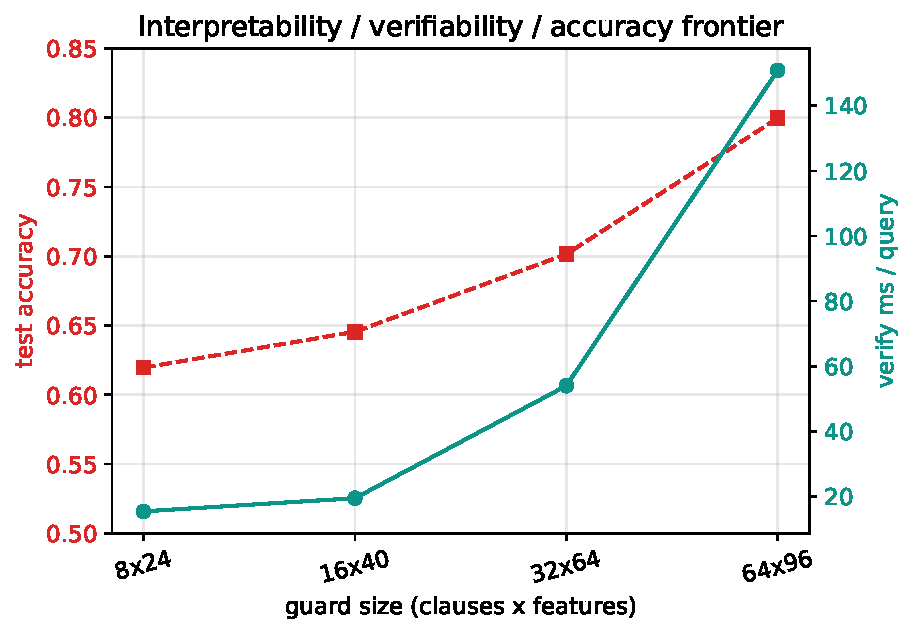
\includegraphics[width=0.49\linewidth]{figures/frontier.pdf}\hfill
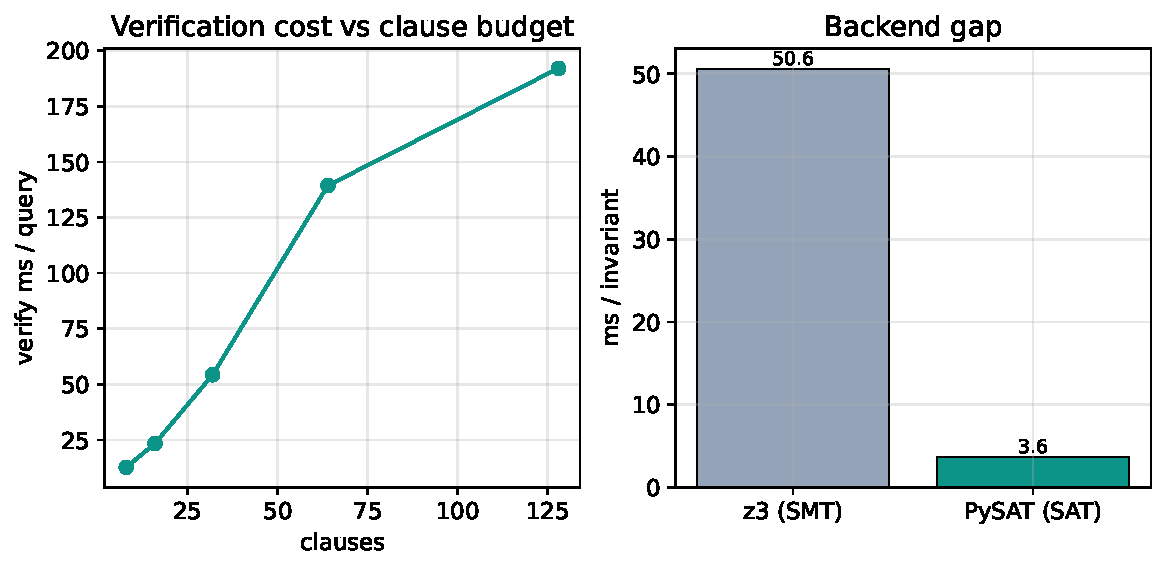
\includegraphics[width=0.49\linewidth]{figures/scaling.pdf}
\caption{E1/E6: (left) the interpretability/verifiability/accuracy frontier, accuracy and verify-time both rise with guard size; (right) verification time vs
clause budget, and the z3-vs-PySAT backend gap.}
\label{fig:frontier}
\end{figure}

\begin{figure}[t]\centering
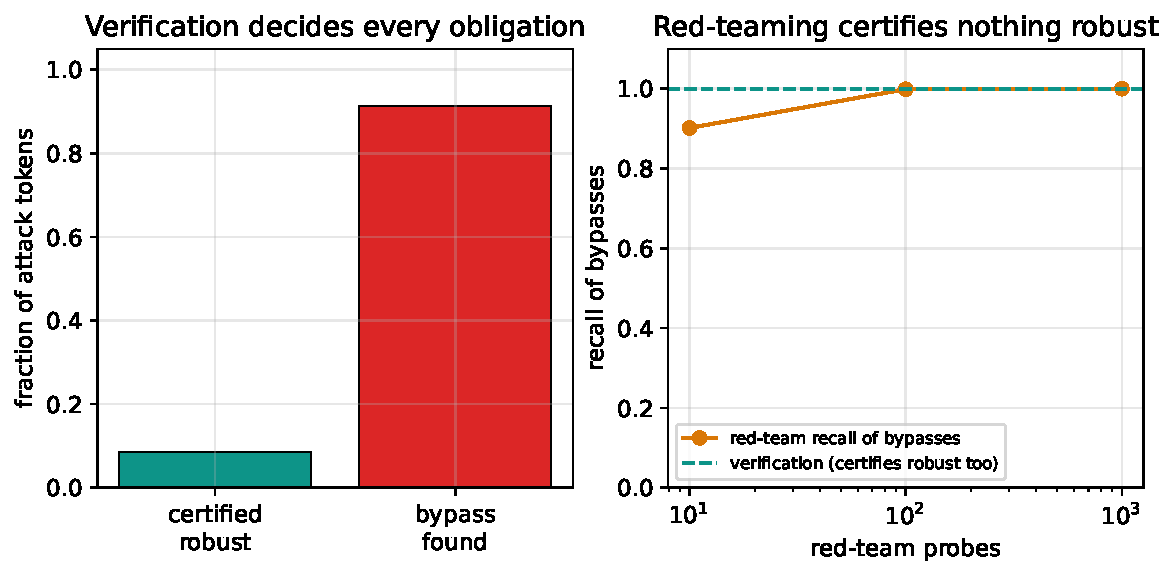
\includegraphics[width=0.49\linewidth]{figures/bypass.pdf}\hfill
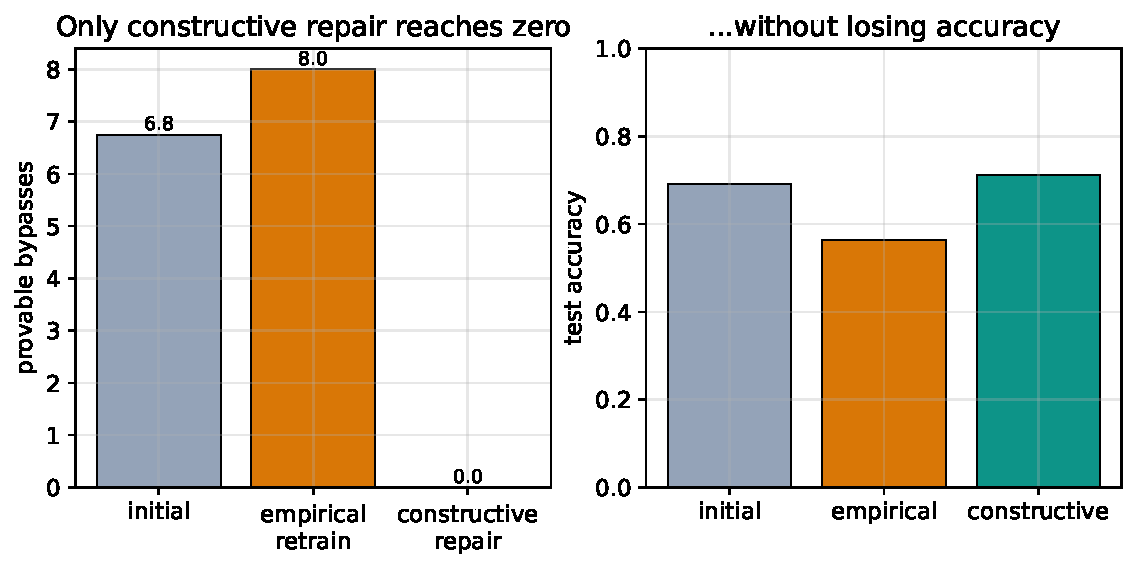
\includegraphics[width=0.49\linewidth]{figures/harden.pdf}
\caption{E2/E3: (left) verification certifies robust tokens and finds every bypass;
red-teaming certifies none. (right) constructive repair drives provable bypasses to
zero where empirical retraining cannot.}
\label{fig:bypass}
\end{figure}

\begin{figure}[t]\centering
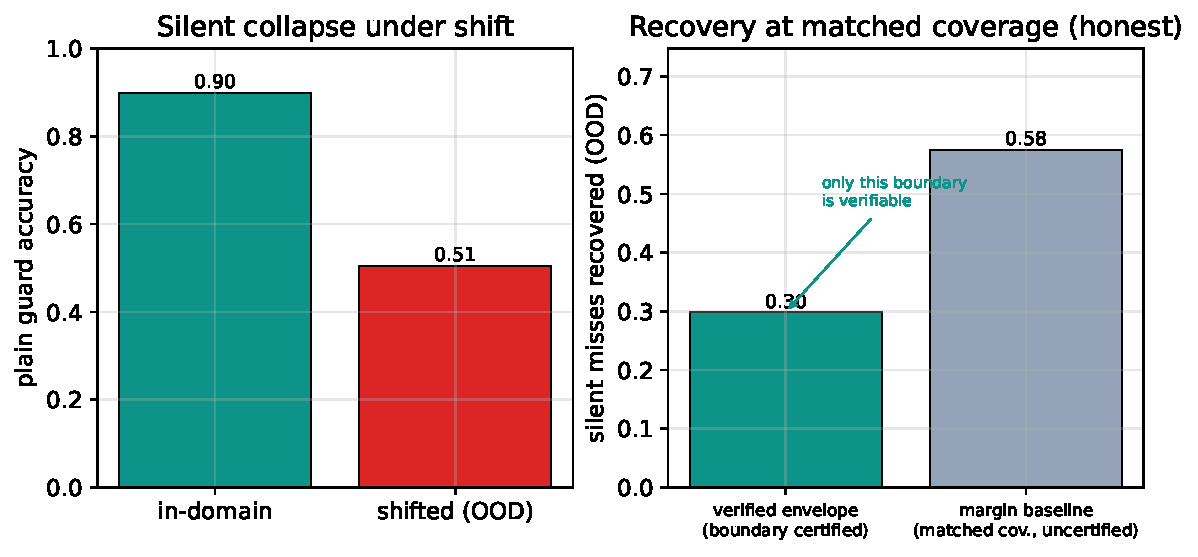
\includegraphics[width=0.6\linewidth]{figures/envelope.pdf}
\caption{E4: (left) under distribution shift the plain guard collapses silently;
(right) the envelope escalates no-cue inputs, recovering some silently-missed
attacks. A coverage-matched uncertified margin baseline recovers \emph{more}; the
envelope's contribution is that its abstention boundary is the only \emph{verifiable}
one (sound in $\soundRate$ of runs), not a higher recovery rate.}
\label{fig:envelope}
\end{figure}

\section{Discussion and limitations}
\label{sec:limits}
\begin{itemize}[leftmargin=1.4em,itemsep=2pt]
\item \textbf{Feature-space verification.} We verify over booleanised feature
vectors, the guard's actual input. A counterexample is a feature vector; mapping it
back to a worst-case \emph{string} (and modelling tokenisation/obfuscation exactly)
is future work, partly addressed by the optional realizability constraints.
\item \textbf{Compact guards.} Verifiability favours small models; our guards trade
accuracy for provability and are not competitive with billion-parameter detectors
on raw accuracy. The frontier (E1) makes the trade-off explicit. Verification cost
grows with size and some large-guard queries would exceed a practical budget.
\item \textbf{Declared properties only.} VERITAS proves what someone wrote a
property for; a harmful behaviour nobody specified is not covered. Trigger-necessity
mitigates this by catching \emph{unspecified} reliance, but property mining is open.
\item \textbf{Repair changes behaviour.} Constructive repair forces a verdict on a
declared token set; for non-attack-exclusive tokens it raises false positives. We
report the cost and recommend it for attack-exclusive obligations.
\item \textbf{Symmetric authentication.} The certificate is HMAC-based;
non-repudiation needs an asymmetric signature over the Merkle root.
\end{itemize}

\section{Ethics and broader impact}
This work is defensive and uses public, Apache-2.0 data with no personal
information. A verified guardrail reduces the false confidence of spot-checked
safety and gives auditors machine-checkable evidence, supporting emerging
obligations~\citep{euaiact2024,dalrymple2024guaranteed}. The interpretable clauses
that make verification possible also reveal the guard's logic to an adversary; we
judge the transparency benefit to outweigh this, consistent with open-source
security practice, and note that a \emph{verified} guard is precisely one whose
exposed logic has no bypass to exploit for the declared class.

\section{Reproducibility}
The repository contains the library, the unit tests (including the bit-exact
encoder check and the three-backend agreement), the six experiments, the figure and
number scripts, the vendored datasets, and this source. \texttt{make test} runs the
suite; \texttt{make reproduce} regenerates every \texttt{results/*.json};
\texttt{make paper} compiles this PDF. The verifier's soundness is itself part of
the test suite.

\section{Conclusion}
A guardrail is a safety component, and a safety component deserves a proof, not a
spot-check. VERITAS shows that when the guard is interpretable, a propositional
Tsetlin Machine, proof is available: we can decide, over all inputs, whether an
attack template bypasses it; we can repair the bypass by construction when it does;
we can make the guard abstain, provably, where it has no competence; and we can seal
the whole assurance argument into a certificate an auditor checks without trusting
us. The exact verification machinery is not ours but
\citeauthor{przybysz2023verifying}'s; the verified, competence-aware guardrail
it makes possible is, we believe, new, and it is the natural completion of an
interpretable agent-safety line whose other pillars detect, certify and enforce.
What remains is string-level verification, property mining, and scaling the
frontier, each a concrete step toward guardrails that are not merely tested but
\emph{accountable}.

\bibliography{references}
\end{document}
